\chapter{Historical Overview\label{ChHist}}
%%%%%%%%%%%%%%%%%%%%%%%%%%%%%%%%%%%%%%%%%%%%%%%%%%%%%%%%%%%%%%%%%%%%%%%%%%%%%%%%%%%%%%%%%
In this chapter we first give a brief overview of scattering at high-energy. We mention the observation, first made by Regge, that the high-energy behavior of the theory in a particular scattering channel determines the bound state spectrum of the theory in a crossed channel. Then we discuss briefly a formalism that uses first-quantization to obtain perturbative scattering amplitudes. We also include a short discussion of the work started by Alday \& Maldacena, involving the use of the AdS/CFT correspondence for the computation of scattering amplitudes at strong coupling.
%%%%%%%%%%%%%%%%%%%%%%%%%%%%%%%%%%%%%%%%%%%%%%%%%%%%%%%%%%%%%%%%%%%%%%%%%%%%%%%%%%%%%%%%%
\section{Regge Scattering\label{ReggeSca}}
%%%%%%%%%%%%%%%%%%%%%%%%%%%%%%%%%%%%%%%%%%%%%%%%%%%%%%%%%%%%%%%%%%%%%%%%%%%%%%%%%%%%%%%%%
In order to be concrete, we will consider the elastic event
\begin{equation}
	a(p_{1}) + b(p_{2}) \longrightarrow a(p_{3}) + b(p_{4}) \label{a1b2a3b4}
\end{equation}
For simplicity, we will assume that a massless scalar field is being exchanged by the massive $a$ and $b$ quanta. The traditional way to study scattering of relativistic matter is to use perturbative quantum field theory\footnote{See \cite{Fields,Srednicki,Sterman} for some textbooks on the subject.}. In this approach, one assumes that the coupling parameter that describes the strength of the interaction is \textit{small}. This allows us to break the event (\ref{a1b2a3b4}) into perturbative contributions, where at lowest order in perturbations one has the least amount of interactions. As the order of perturbation increases, one consider more complicated events with greater number of interactions. With the aid of Feynman graphs, one can assign a picture to each of these perturbative contributions.

At lowest order in perturbations, the only connected Feynman graph is
\begin{equation}
	\vcenter{\hbox{\includegraphics[scale=0.4]{Figures/TreeSChannel.pdf}\put(-55,50){$1$} \put(-61,-2){$2$} \put(3,50){$3$} \put(-3,-4){$4$}}} \label{a1b2a3b4Tree}
\end{equation}
Since this graph has no loops, it is referred to a the tree graph. The tree graph translates to the expression
\begin{equation}
	{-\frac{\alpha}{t}} \delta(p_{1} + p_{2} - p_{3} - p_{4})
\end{equation}
Here $\alpha$ is the coupling parameter and $t = -(p_{1} - p_{3})^{2}$ parametrizes the momentum transfer between the two external states. The Dirac delta is in charge of making sure that the total momentum that is incoming (given by $p_{1} + p_{2}$) equals the total momentum that is outgoing (given by $p_{3} + p_{4}$).

The next order in perturbations involve many contributions. For our discussion, the relevant contributions come from the box graph and the crossed box graph:
\begin{equation}
	\vcenter{\hbox{\includegraphics[scale=0.4]{Figures/BoxSChannel.pdf}\put(-87,50){$1$} \put(-93,-2){$2$} \put(3,50){$3$} \put(-3,-4){$4$}}} \qquad \qquad \qquad \vcenter{\hbox{\includegraphics[scale=0.4]{Figures/CrossedBoxSChannel.pdf}\put(-87,50){$1$} \put(-93,-2){$2$} \put(3,50){$3$} \put(-3,-4){$4$}}} \label{a1b2a3b4Boxes}
\end{equation}
These graphs are examples of ladder graphs. Other examples include
\begin{equation}
	\vcenter{\hbox{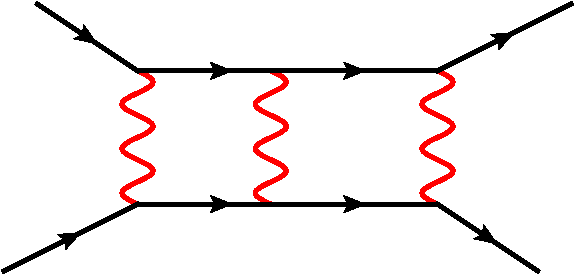
\includegraphics[scale=0.4]{Figures/Ladder2SChannel.pdf}\put(-113,50){$1$} \put(-118,-2){$2$} \put(3,50){$3$} \put(-3,-4){$4$}}} \qquad \qquad \qquad \vcenter{\hbox{\includegraphics[scale=0.4]{Figures/Ladder3SChannel.pdf}\put(-143,50){$1$} \put(-150,-2){$2$} \put(3,50){$3$} \put(-3,-4){$4$}}}
\end{equation}
Each of the graphs in (\ref{a1b2a3b4Boxes}) has one closed loop, so they are referred to as one-loop graphs. The box graph translates to the expression
\begin{equation}
	\alpha^{2} \int\limits_{0}^{1} \int\limits_{0}^{1} \int\limits_{0}^{1} \int\limits_{0}^{1} \mathrm{d}f_{31} \mathrm{d}f_{42} \mathrm{d}f_{12} \mathrm{d}f_{34} \left[ \frac{\delta(1 - f_{12} - f_{34} - f_{31} - f_{42})}{B(s, t|f_{ij})} \right] \label{BoxExpr}
\end{equation}
with
\begin{equation}
	B(s, t|f_{ij}) = m_{a}^{2} f_{31}^{2} + m_{b}^{2} f_{42}^{2} + (m_{a}^{2} + m_{b}^{2} - s) f_{31} f_{42} - t f_{12} f_{34}
\end{equation}
Here $s = -(p_{1} + p_{2})^{2}$ parametrizes the squared center-of-momentum energy. Expression (\ref{BoxExpr}) is valid for \textit{generic} values of the kinematical variables $s$ and $t$, as long as they are \textit{inside} of the physical scattering region (see appendix \ref{AppKin4}). However, the contribution from the box graph involves a nontrivial integration. With considerable effort, the integrals can be evaluated exactly \cite{tHVelt,Denner:1991qq}.

At higher-orders in perturbations, the challenges are much greater. In the face of inherent mathematical difficulties, one can always use approximations. One type of approximation involves restricting to a certain kinematical regime. For example, we can study the limit $t \rightarrow \infty$ while keeping $s$, and the masses $m_{a}$ and $m_{b}$, fixed. At first glance, this limit appears to be in the wrong direction: $t$ is negative inside of the physical scattering region! If we want to study scattering phenomena, it makes a lot of sense to stay inside of the physical scattering region. But the $t \rightarrow \infty$ limit allows us to study another kind of phenomena.

Besides the scattering event (\ref{a1b2a3b4}), we can also have the event
\begin{equation}
	a(p_{1}) + \bar{a}(\bar{p}_{2}) \longrightarrow \bar{b}(\bar{p}_{3}) + b(p_{4}) \label{a1a2b3b4}
\end{equation}
The Feynman graphs for this event are related to the graphs for event (\ref{a1b2a3b4}) by a rotation and a relabelling of the external states:
\begin{equation}
	\vcenter{\hbox{\includegraphics[scale=0.4]{Figures/TreeTChannel.pdf}\put(-87,23){$1$} \put(-94,-2){$\bar{2}$} \put(3,23){$\bar{3}$} \put(-3,-4){$4$}}}
\end{equation}
Indeed, event (\ref{a1a2b3b4}) follows from event (\ref{a1b2a3b4}) after crossing the incoming $b$ state with the outgoing $a$ state, and setting
\begin{equation}
	\bar{p}_{2} = -p_{3}, \qquad \bar{p}_{3} = -p_{2}
\end{equation}
For event (\ref{a1a2b3b4}), the center-of-momentum energy is
\begin{equation}
	\bar{s} = -(p_{1} + \bar{p}_{2})^{2} = -(p_{1} - p_{3})^{2} = t
\end{equation}
and the momentum transfer is
\begin{equation}
	\bar{t} = -(p_{1} - \bar{p}_{3})^{2} = -(p_{1} + p_{2})^{2} = s
\end{equation}
Thus, we can use the same kinematical variables (the four momentum vectors $p_{j}$) to describe both events (\ref{a1b2a3b4}) and (\ref{a1a2b3b4}). However, the physical scattering region for each event do not overlap: $\bar{s} > 0$ implies $t > 0$ in event (\ref{a1a2b3b4}), but $t < 0$ in event (\ref{a1b2a3b4}). In particular, the high-energy limit $\bar{s} \rightarrow \infty$ corresponds to the unphysical limit $t \rightarrow \infty$ that we mentioned earlier. The cosine of the scattering angle in event (\ref{a1b2a3b4}) is
\begin{equation}
	z_{s} \equiv \cos{(\theta_{s})} = 1 + \frac{2 s t}{[s - (m_{a} - m_{b})^{2}] [s - (m_{a} + m_{b})^{2}]}
\end{equation}
Thus, $z_{s} \rightarrow \infty$ as $t \rightarrow \infty$. This suggest that the scattering angle $\theta_{s}$ becomes \textit{complex}, which leads one to believe that the corresponding conjugate variable to the scattering angle, the angular momentum, also becomes complex. This argument lead Regge to promote the orbital angular momentum in quantum mechanics to a complex variable \cite{Regge:1959mz,Regge:1960zc}.

In the $\bar{s} \rightarrow \infty$ limit, one can use asymptotic methods to evaluate some of the integrals in (\ref{BoxExpr}):
\begin{equation}
	\frac{\alpha}{t} [ \alpha \rho(\bar{t})] \log{\left( \frac{\bar{s}}{2 \mu^{2}} \right)} \label{BoxExprEval}
\end{equation}
where
\begin{equation}
	\rho(\bar{t}) = \int\limits_{0}^{1} \frac{\mathrm{d}f}{m_{b}^{2} + (m_{a}^{2} - m_{b}^{2} - \bar{t})f + \bar{t} f^{2}}
\end{equation}
(This result is only valid in $D = 4$.) Indeed, (\ref{BoxExprEval}) agrees with the \textit{exact} result for the scalar box with elastic kinematics, which can be found in \cite{PvN}. For longer ladder graphs, the $\bar{s} \rightarrow \infty$ limit no longer yields the exact answer, but one can still obtain the leading behavior in the $\bar{s} \rightarrow \infty$ limit. After adding all ladder contributions \cite{LeeSawyer}, one obtains
\begin{equation}
	\alpha \Gamma[-R(\bar{t})] \left( \frac{\bar{s}}{2 \mu^{2}} \right)^{R(\bar{t})}, \qquad R(\bar{t}) = -1 + \alpha \rho(\bar{t})
\end{equation}
with $R(\bar{t})$ being complex. When an amplitude takes this form, it is said to show Regge behavior. This result corresponds to the \textit{high-energy} ($\bar{s} \rightarrow \infty$) behavior of the ladder series for the event (\ref{a1a2b3b4}). But, by analytic continuation to the event (\ref{a1b2a3b4}), the same result corresponds to an amplitude outside of the physical scattering region ($t \rightarrow \infty$, or $z_{s} \rightarrow \infty$). In this region, the singularities of the Euler Gamma function are accessible, and thus correspond to physical states in the theory. These singularities are identified as bound states. Thus, the high-energy behavior of the scattering amplitude in one scattering event is responsible for the formation of bound states in another scattering event, related to the former by crossing. This is the main idea behind Regge theory.

The previous discussion is meant as a quick introduction to Regge scattering and the Regge limit. Since Regge theory yields information about the spectrum of bound states, it has direct phenomenological and experimental relevance. The topic is vast, and we do not have the time or the space to cover it properly. The curious reader may consult textbooks on Regge theory \cite{Collins,Gribov}, textbooks on high-energy scattering \cite{ChengWuBook,Eden,SMatrixBook} and reviews \cite{Hite:1969td,Collins:1971ff,Eden:1971jm,Brower:1974yv,Irving:1977ea} for more details.
%%%%%%%%%%%%%%%%%%%%%%%%%%%%%%%%%%%%%%%%%%%%%%%%%%%%%%%%%%%%%%%%%%%%%%%%%%%%%%%%%%%%%%%%%
\section{Perturbative First-Quantization\label{SecPert1stQuant}}
%%%%%%%%%%%%%%%%%%%%%%%%%%%%%%%%%%%%%%%%%%%%%%%%%%%%%%%%%%%%%%%%%%%%%%%%%%%%%%%%%%%%%%%%%
We use first-quantized path integrals (i.e. functional integrals over mechanical variables, like paths) to compute nonperturbative scattering amplitudes. In this section we briefly discuss a formalism that uses first-quantization to compute \textit{perturbative} scattering amplitudes.

Let us consider the following event: a massive scalar particle $a$ with incoming momentum $p_{I}$ and outgoing momentum $p_{O}$ moves in spacetime and emits $N$ massless scalar quanta. The $n$-th emitted massless quanta carries momentum $k_{n}$. At tree level, we can describe this event with the quantum mechanical amplitude
\begin{equation}
	\mathcal{S}_{T}(O|I) = g^{N} \langle p_{O} | V(k_{N}) \cdots V(k_{2}) V(k_{1}) | p_{I} \rangle
\end{equation}
Here $V(k_{n})$ is a vertex operator that describes the emission of the $n$-th massless quanta and $g$ is the coupling parameter. This amplitude can be rewritten as a path integral,
\begin{equation}
	\mathcal{S}_{T}(O|I) = g^{N} \int \int \mathrm{d}x_{I} \mathrm{d}x_{O} \, \overline{\mathcal{W}}_{O} \mathcal{W}_{I} \int\limits_{x_{I}}^{x_{O}} \mathrm{D}q_{a}(\tau) \, \exp{\left( -i S_{J}[q_{a}] \right)} \label{eq318}
\end{equation}
where
\begin{equation}
	\mathcal{W}_{I} \equiv \exp{(i x_{I} \cdot p_{I})} \qquad \overline{\mathcal{W}}_{O} \equiv \exp{(-i x_{O} \cdot p_{O})}
\end{equation}
and the action functional $S_{J}$ is given by
\begin{equation}
	S_{J}[q_{a}] = \int \mathrm{d}\tau \left[ -\frac{1}{2}\dot{q}_{a}^{2} + \frac{1}{2}m_{a}^{2} - J \cdot q_{a} \right]
\end{equation}
with the source $J$ given by
\begin{equation}
	J(\tau) = -\sum_{n = 1}^{N} k_{n} \delta(\tau - \tau_{n})
\end{equation}
Note that
\begin{equation}
	\tau_{I} < \tau_{1} < \tau_{2} < \ldots < \tau_{N} < \tau_{O}
\end{equation}
The path integral in (\ref{eq318}) can be evaluated \textit{exactly} by using the semiclassical approximation. This involves finding the classical solution $q_{*}(\tau)$ by solving
\begin{equation}
	\ddot{q}_{*} = J, \qquad q_{*}(\tau_{I}) = x_{I}, \qquad q_{*}(\tau_{O}) = x_{O}
\end{equation}
and evaluating the action functional $S_{J}$ at this classical solution. After obtaining the semiclassical path integral, and integrating over the $N + 1$ moduli
\begin{equation}
	T_{1I} = \tau_{1} - \tau_{I}, \qquad T_{21} = \tau_{2} - \tau_{1}, \qquad \ldots \qquad T_{ON} = \tau_{O} - \tau_{N}
\end{equation}
one recovers, after truncating two external $a$ propagators, the familiar expression for an $(N+2)$-point tree level scattering amplitude with $N - 1$ simple poles at $m_{a}^{2}$. For external scalars, this procedure might seem like a complicated way to obtain a tree level amplitude. The formalism can be applied to external states with spin and yields tree level amplitudes with arbitrary number of external states \cite{Kosower:1987ic}. Indeed, this formalism is inspired by the methods used in string theory to compute scattering amplitudes \cite{GSW1,Polchinski1,Fields}. Similar ideas can be used to compute one-loop amplitudes \cite{
Bern:1990cu,Bern:1991aq,Bern:1991an,Roland:1992cc,Strassler:1992zr,Schubert:2001he}.

While this formalism allows efficient \textit{exact} computations, the results are still \textit{perturbative}. One can argue that this formalism uses a classical solution to compute perturbative scattering amplitudes, and thus the semiclassical approximation does not necessarily leads to strong-coupling dynamics. This is somewhat misleading: the path integral (\ref{eq318}) is Gaussian and hence the exact value happens to coincide with the semiclassical path integral.
%%%%%%%%%%%%%%%%%%%%%%%%%%%%%%%%%%%%%%%%%%%%%%%%%%%%%%%%%%%%%%%%%%%%%%%%%%%%%%%%%%%%%%%%%
\section{Alday-Maldacena Theory}
%%%%%%%%%%%%%%%%%%%%%%%%%%%%%%%%%%%%%%%%%%%%%%%%%%%%%%%%%%%%%%%%%%%%%%%%%%%%%%%%%%%%%%%%%
The AdS/CFT correspondence \cite{Maldacena:1997re} provides a relation between two different theories: the four-dimensional conformal field theory $\mathcal{N} = 4$ super Yang-Mills theory with gauge group $SU(N_{c})$, and the ten-dimensional type IIB superstring theory in $AdS_{5} \times S^{5}$ with $N_{c}$ units of Ramond-Ramond five-flux (see \cite{Aharony:1999ti} for a review). This relation is a ``duality'': it relates the \textit{planar strong-coupling} regime of the CFT to the \textit{semiclassical} regime of the superstring theory.

Alday \& Maldacena \cite{Alday:2007hr} proposed a way to compute four-point scattering amplitudes of gluons in $\mathcal{N} = 4$ SYM at strong-coupling, by using classical solutions of strings in $AdS_{5}$. As a string moves in $AdS_{5}$, it traces a surface in spacetime. Thus, solving the classical equations of motion for a string involves searching for a surface of minimal area in $AdS_{5}$. The scattering regime that Alday \& Maldacena consider is \textit{fixed-angle scattering}, where one takes all the kinematical variables to be very large while keeping all the ratios fixed (and thus, keeping the scattering angle fixed). Indeed, this calculation in $AdS_{5}$ is a generalization of a calculation done much earlier in flat spacetime \cite{Gross:1987kza,Gross:1987ar,Gross:1989ge}.

As usual in string theory, the kinematical information of the external states is encoded in the boundary conditions of the classical solution. In the naive formulation of the problem, it seems hopeless to find a minimal surface in $AdS_{5}$ with the required boundary conditions (four punctures where external momentum is inserted into the worldsheet).

But Alday \& Maldacena realized that after a change of variables (analogous to a noncompact T-duality), one could re-formulate the problem in terms of different boundary conditions. In terms of the new variables, the minimal surface ends on a particular polygon in spacetime with four lightlike edges, each corresponding to the external momentum of a gluon. This lightlike polygon was later identified with a Wilson loop living on the boundary of $AdS_{5}$. The classical string solution was found, and, after introducing a regulator to deal with infrared divergences, the area of the classical string solution (i.e. the minimal action) was shown to agree with a previous ansatz of Bern, Dixon \& Smirnov \cite{Bern:2005iz} for the planar MHV scattering amplitude with four gluons.

The work of Alday \& Maldacena uncovered a connection between planar MHV amplitudes and expectation values of Wilson loops (see \cite{Alday:2008yw,Alday:2010kn} for reviews). The change of variables that leads to the formulation of the problem in terms of the lightlike polygon signalled the existence of another copy of conformal symmetry, now referred to as \textit{dual conformal symmetry}. The invariants of this symmetry are conformal ratios that involve momentum variables. This in turn lead to the realization that planar scattering amplitudes in $\mathcal{N} = 4$ SYM enjoy an infinite-dimensional symmetry in the guise of a Yangian \cite{Berkovits:2008ic,Drummond:2009fd}.

Further work includes higher-point amplitudes \cite{Alday:2007mf,Alday:2007he}, where it was found that the BDS ansatz was incomplete, since it failed to account for dual conformal symmetry. Other work makes use of integrable systems on the worldsheet to study amplitudes with any number of external gluons \cite{Alday:2009yn,Alday:2009dv,Alday:2010vh}, the development of an operator product expansion for the perturbative study of lightlike Wilson loops \cite{Alday:2010ku,Gaiotto:2010fk,Gaiotto:2011dt}, form factors at strong-coupling \cite{Maldacena:2010kp}, and a study of the cusp anomalous dimension \cite{Correa:2012at,Correa:2012nk,Correa:2012hh}.

Quark scattering was also studied, both massless \cite{Komargodski:2007er,McGreevy:2007kt} and massive \cite{Barnes:2009ag}. In light of the results presented in this dissertation, the amplitude with quarks might be more relevant than the amplitude with gluons. The work in this dissertation started as an attempt to generalize Alday-Maldacena theory to other cases. We are still nowhere ready to do that. Indeed, we might even be late to the party \cite{Giordano:2011ua}. Earlier work on scattering amplitudes via AdS/CFT include \cite{Rho:1999jm,Janik:1999zk,Janik:2000aj}. These references might be important and/or useful in developing a more general formalism that does not rely on the specific details of the Alday-Maldacena setup.